\otazka{5. Síťové aplikace a bezpečnost}{Základní aplikační protokoly: doručování pošty, přenos souborů, web, jmenná služba. Principy popisu a zajištění kvality služby, použití pro multimédia. Zabezpečení síťové komunikace, autentizace a šifrování, zabezpečení na jednotlivých protokolových vrstvách.}{PB156}

\subsection*{5. Síťové aplikace a bezpečnost -- stručněji}
Tahle otázka navazuje na sítě: už neřeší jen doručení paketů, ale konkrétní služby pro uživatele, jejich požadavky na kvalitu a způsoby zabezpečení komunikace.

\textbf{1. Aplikační protokoly}
\begin{itemize}
  \item Web stojí hlavně na HTTP/HTTPS. HTTP je aplikační protokol pro požadavky a odpovědi, HTTPS znamená HTTP chráněné TLS.
  \item DNS překládá doménová jména na IP adresy a další záznamy. Je kritické, protože když selže DNS, uživatel často neví, kam se připojit.
  \item E-mail používá SMTP pro odesílání mezi servery, IMAP nebo POP3 pro přístup ke schránce. Bezpečnost doplňují SPF, DKIM a DMARC proti spoofingu.
  \item Přenos souborů může používat FTP, SFTP, SCP nebo HTTPS. Důležité je rozlišit staré nešifrované protokoly od variant chráněných SSH nebo TLS.
\end{itemize}

\textbf{2. Kvalita služby a multimédia}
\begin{itemize}
  \item QoS popisuje požadavky na přenos: latence, jitter, ztrátovost, propustnost a dostupnost.
  \item Multimédia často snesou malou ztrátu paketů, ale špatně snášejí vysokou latenci a jitter. Proto je u VoIP nebo videohovorů důležitější plynulost než dokonalé opakování každého paketu.
\end{itemize}

\textbf{3. Bezpečnost komunikace}
\begin{itemize}
  \item Bezpečnost řeší důvěrnost, integritu, autentizaci a někdy nepopiratelnost. Nejčastější praktický nástroj je TLS nad transportní vrstvou.
  \item Autentizace serveru v TLS stojí na certifikátu a důvěryhodné certifikační autoritě. Klient tím ověřuje, že mluví se správným serverem.
  \item Na různých vrstvách existují různé nástroje: WPA2/WPA3 na Wi-Fi/linkové vrstvě, IPsec na síťové vrstvě, TLS na transportně-aplikační hranici, aplikační podpisy a tokeny přímo v aplikaci.
\end{itemize}

\textbf{4. Typické zkouškové rozlišení}
\begin{itemize}
  \item TLS chrání spojení mezi koncovými body, ale neřeší, zda aplikace uvnitř správně autorizuje uživatele.
  \item VPN chrání síťový přístup, ale nenahrazuje aplikační autentizaci, logování a řízení oprávnění.
  \item Šifrování zajišťuje důvěrnost, hash integritu, podpis integritu plus vazbu na podepisujícího a certifikát váže veřejný klíč na identitu.
\end{itemize}

služby, použití pro multimédia. Zabezpečení síťové komunikace, \textbf{autentizace} a šifrování, zabezpečení na jednotlivých protokolových vrstvách.

Tento text je napsaný jako souvislé opakování: cílem není naučit se nazpaměť seznam protokolů, ale umět u státnic popsat, co se na aplikační vrstvě děje, jaké služby se typicky používají, co od sítě požadují multimédia a kde se dá komunikace zabezpečit. Důležité je držet rozdíl mezi aplikačním protokolem, transportním protokolem, bezpečnostní nadstavbou a konkrétní službou pro uživatele.

\subsection*{1. Síťové aplikace a aplikační protokoly}

Síťová aplikace je program nebo služba, která využívá síť ke komunikaci s jinou aplikací. Patří do aplikační vrstvy, tedy do vrstvy, která je nejblíže uživateli nebo aplikační logice. Aplikační protokol potom definuje, jak si aplikace budou rozumět: jaké typy zpráv se posílají, jakou mají syntaxi, jaký je význam jednotlivých částí zprávy a kdy se mají odesílat odpovědi.

Protokol je tedy dohoda o jazyce komunikace. \textbf{HTTP} říká, jak má vypadat požadavek na webovou stránku, \textbf{SMTP} říká, jak se předává pošta, \textbf{DNS} říká, jak se ptát na překlad jména na IP adresu.

Z hlediska komunikačního modelu se často rozlišuje model klient-server a peer-to-peer. V modelu klient-server komunikaci iniciuje klient, typicky prohlížeč, poštovní klient nebo \textbf{FTP} klient, a server poskytuje službu. Výhodou je centralizace a jednodušší správa, nevýhodou závislost na serveru.

Peer-to-peer je decentralizovanější: uzly jsou zároveň klienty i poskytovateli zdrojů, což známe například ze sdílení souborů nebo některých komunikačních systémů. Podle směru iniciace dat lze rozlišit pull model, kde si klient data vyžádá, typicky web, a push model, kde server posílá data podle profilu nebo předchozího přihlášení, typicky notifikace nebo některé formy streamingu.

Aplikační protokoly typicky běží nad \textbf{TCP} nebo \textbf{UDP}. Nad TCP běží například HTTP/\textbf{HTTPS}, FTP, SMTP, \textbf{POP3}, \textbf{IMAP}, \textbf{SSH} nebo Telnet, protože často potřebují spolehlivý proud dat. Nad UDP běží například DNS dotazy, \textbf{DHCP}, TFTP nebo multimediální protokoly, kde je někdy výhodnější nízká režie a rychlost než čekání na znovuodeslání každého ztraceného paketu.

Některé služby používají oba transportní protokoly podle situace, například DNS běžně UDP/53 pro dotazy, ale TCP/53 pro větší odpovědi nebo zónové přenosy.

\itbox{\textbf{Státnicová věta:} Aplikační protokol definuje formát a význam zpráv mezi aplikacemi; transportní protokol pod ním řeší, jak se data dostanou mezi procesy. SMTP, HTTP nebo DNS tedy nejsou totéž co TCP nebo UDP - používají je jako transportní službu.}

\subsection*{2. Doručování pošty: SMTP, POP3, IMAP, TLS, PGP/S-MIME}

U elektronické pošty je zásadní neplést odesílání a vyzvedávání. SMTP slouží k odesílání a předávání pošty. Používá se při odeslání zprávy z klienta na poštovní server a hlavně při předávání mezi poštovními servery. Pro komunikaci mezi poštovními servery se historicky používá port 25/TCP, pro odesílání od klienta se často používá port 587/TCP se zabezpečením a autentizací.

SMTP zpráva má obálku, podle které se doručuje, a vlastní zprávu, která má hlavičky a tělo. Hlavičky obsahují například From, To, Subject a další metadata, tělo obsahuje vlastní obsah zprávy.

Doručení zprávy si lze představit ve třech krocích. Nejprve poštovní klient nebo odesílající systém předá zprávu lokálnímu poštovnímu serveru pomocí SMTP. Tento server podle domény příjemce zjistí cílový poštovní server, typicky přes DNS záznamy typu MX, a opět SMTP protokolem mu zprávu předá. Nakonec si cílový uživatel zprávu vyzvedává nebo synchronizuje pomocí POP3 nebo IMAP.

POP3 je jednodušší protokol pro stažení pošty ze serveru do klienta. Běží typicky na TCP portu 110, zabezpečená varianta POP3S na portu 995. V klasickém modelu se zprávy stáhnou do klienta a mohou se ze serveru mazat, což umožňuje offline práci, ale hůř se hodí pro více zařízení. IMAP, aktuálně IMAP4, slouží ke vzdálenému přístupu ke schránce.

Zprávy a složky zůstávají na serveru, klient si stahuje hlavičky a obsah až podle potřeby, stav zpráv jako přečtená/nepřečtená se synchronizuje a více klientů může pracovat současně. IMAP běží typicky na TCP portu 143, IMAPS na 993.

Bezpečnost pošty má dvě různé roviny. První je zabezpečení přenosu mezi klientem a serverem nebo mezi servery pomocí \textbf{TLS}. To chrání data na daném úseku přenosu, ale poštovní server zprávu může vidět. Druhá rovina je end-to-end zabezpečení obsahu zprávy, například \textbf{PGP} nebo \textbf{S/MIME}.

PGP kombinuje symetrickou a asymetrickou kryptografii: obsah se zašifruje rychlou symetrickou šifrou, symetrický klíč se zašifruje veřejným klíčem příjemce a odesílatel může zprávu podepsat svým soukromým klíčem. Tím se řeší \textbf{důvěrnost}, \textbf{integrita}, autentizace odesílatele a nepopíratelnost. S/MIME řeší podobnou oblast, ale více stojí na \textbf{X.509} certifikátech a certifikačních autoritách.

S poštou souvisí ještě tři mechanismy proti podvržení odesílatele, které je dobré nezaměňovat se šifrováním obsahu. \textbf{SPF} (Sender Policy Framework) v DNS určuje, které servery smí odesílat poštu za danou doménu, takže příjemce pozná zprávu z neoprávněného serveru. \textbf{DKIM} (DomainKeys Identified Mail) přidává ke zprávě \textbf{digitální podpis} hlaviček klíčem domény, čímž ověří, že zpráva za doménu opravdu prošla a cestou se nezměnila. \textbf{DMARC} nad tím staví politiku: říká, jak se zachovat, když SPF nebo DKIM neprojde (například zprávu odmítnout nebo dát do spamu), a umožňuje reporting.

Tyto mechanismy ověřují legitimitu odesílající domény, ale neřeší end-to-end šifrování obsahu zprávy; na to slouží PGP nebo S/MIME.

\itbox{\textbf{Pohlídat:} SMTP = odesílání/předávání pošty. POP3/IMAP = vyzvedávání/synchronizace schránky. TLS chrání kanál, PGP/S-MIME chrání obsah zprávy end-to-end.}

\subsection*{3. Přenos souborů: FTP, FTPS a SFTP}

FTP je starý internetový protokol pro přenos souborů mezi klientem a serverem. Umožňuje přihlášení, práci s adresáři, výpis souborů, upload, download a volbu typu přenosu. Zvláštnost FTP je, že používá dvě TCP spojení: řídicí spojení typicky na portu 21, které trvá po dobu relace a přenáší příkazy a odpovědi, a datové spojení, které se otevírá pro vlastní přenos souboru nebo výpis adresáře.

Historicky se pro datové spojení uvádí port 20, ale v praxi existuje aktivní a pasivní režim, což je důležité kvůli firewallům a \textbf{NAT}.

Klasické FTP není bezpečné, protože přenáší přihlašovací údaje i data bez šifrování. \textbf{FTPS} znamená FTP zabezpečené pomocí TLS/\textbf{SSL}.

Je to tedy původní FTP protokol, ale zabalený do TLS, typicky explicitně na portu 21 nebo implicitně historicky na portu 990. \textbf{SFTP} je něco jiného: není to FTP přes TLS, ale samostatný protokol pro přenos souborů nad SSH, typicky na portu 22. U zkoušky je důležité explicitně říct, že FTPS a SFTP nejsou totéž. FTPS = FTP + TLS; SFTP = přenos souborů přes SSH.

\subsection*{4. Web: HTTP, HTTPS, URL, stav a cookies}

Internet je síť sítí postavená na rodině protokolů \textbf{TCP/IP}. Web je pouze jedna ze služeb běžících na Internetu. Web používá dokumenty a zdroje adresované pomocí URL a přenášené protokolem HTTP. HTTP je aplikační protokol typu dotaz-odpověď: klient, typicky webový prohlížeč, odešle požadavek a server vrátí odpověď.

HTTP běží typicky nad TCP portem 80 a HTTPS typicky nad TCP portem 443. HTTPS není nový aplikační protokol ve smyslu jiné sémantiky webu; je to HTTP komunikace chráněná pomocí TLS.

HTTP existuje ve více verzích, které se liší hlavně výkonem, ne významem. HTTP/1.1 zavedl \textbf{perzistentní spojení} (keep-alive): jedno TCP spojení se znovu použije pro více požadavků, místo aby se otevíralo nové pro každý objekt. HTTP/2 přidal \textbf{multiplexing}: po jednom spojení může současně běžet více nezávislých streamů, takže se pomalý požadavek nezasekne za ostatními.

HTTP/3 jde dál a místo TCP používá protokol \textbf{QUIC} postavený nad UDP, který si spolehlivost a multiplexing řeší sám a rychleji navazuje šifrované spojení. Právě proto neplatí absolutně, že HTTPS vždy běží nad TCP: u HTTP/3 běží nad UDP.

URL určuje, jaký zdroj chce klient získat. Obsahuje schéma/protokol, například https, jméno hostitele, volitelně port, cestu a případně parametry. HTTP samo o sobě je bezstavové: jednotlivé požadavky na sebe protokolově nenavazují. Pokud chce webová aplikace udržet přihlášení, košík nebo stav relace, používá mechanismy nad HTTP, typicky cookies, session identifikátory nebo tokeny.

Webové dokumenty mohou být statické, tedy uložené soubory, dynamické, tedy generované serverem podle požadavku, nebo aktivní, kdy server pošle kód spouštěný na klientovi, typicky JavaScript.

TLS u HTTPS poskytuje autentizaci serveru pomocí certifikátu, dohodu klíčů a šifrování následné komunikace. Klient v handshake pošle podporované verze a šifry, server odpoví certifikátem a parametry, klient ověří \textbf{certifikát} vůči důvěryhodným certifikačním autoritám a obě strany si odvodí symetrické klíče pro vlastní přenos. Praktický význam: útočník na cestě nemá vidět obsah ani ho nemá umět nepozorovaně změnit.

TLS ale neznamená, že provozovatel serveru zachází s daty bezpečně po jejich dešifrování.

Podrobněji probíhá \textbf{TLS handshake} takto:
\begin{enumerate}
  \item \textbf{ClientHello} -- klient pošle podporované verze, šifry a náhodná data.
  \item \textbf{ServerHello} -- server odpoví vybranými parametry a pošle svůj \textbf{certifikát}, obvykle spolu s certifikačním řetězcem vedoucím od certifikátu serveru přes mezilehlé autority až ke kořenové certifikační autoritě (root CA), které klient důvěřuje.
  \item \textbf{Ověření certifikátu} -- klient zkontroluje platnost (datum, případné zneplatnění) a hlavně to, že jméno v certifikátu odpovídá hostname, na který se připojuje.
  \item \textbf{Dohoda klíčů} -- strany si pomocí efemérního Diffie-Hellmana (ephemeral DH) dohodnou sdílené tajemství a z něj odvodí symetrické klíče.
  \item \textbf{Šifrovaný přenos} -- další data už přenášejí rychlou symetrickou šifrou v režimu \textbf{AEAD}, který zároveň zajišťuje důvěrnost i integritu.
\end{enumerate}

Je důležité zdůraznit, že certifikát neslouží k šifrování celého přenosu; jen váže identitu serveru k jeho veřejnému klíči, a tím umožní klientovi ověřit, s kým mluví. Vlastní šifrování zajišťují až odvozené symetrické klíče.

U samotné symetrické (blokové) šifry je dobré znát i provozní režimy. \textbf{ECB} (Electronic Codebook) šifruje každý blok nezávisle stejným klíčem, takže stejný blok otevřeného textu dá vždy stejný šifrovaný blok -- tím prozrazuje vzory v datech a je nebezpečný. \textbf{CBC} (Cipher Block Chaining) každý blok před zašifrováním zkombinuje (XOR) s předchozím zašifrovaným blokem a první blok s náhodným inicializačním vektorem (IV), takže i stejné bloky dají různý výstup; je bezpečnější, ale šifruje sériově. Moderní režimy navíc rovnou přidávají i autenticitu (AEAD, například AES-GCM).

\subsection*{5. DNS: jmenná služba, hierarchie a resolver}

DNS je distribuovaná hierarchická jmenná služba pro překlad doménových jmen na IP adresy a zpět. Lidé si pamatují jména jako aisa.fi.muni.cz, stroje směrují podle IP adres. DNS běží na UDP/53 i TCP/53. Doménový jmenný prostor má tvar obráceného stromu. Úplně nahoře je kořen, pod ním domény nejvyšší úrovně, tedy TLD, například .cz, .com, .org, a pod nimi jednotlivé domény a subdomény.

Registrátor je subjekt, přes kterého si držitel registruje doménu u příslušného registru TLD.

Praktické vyřešení dotazu obvykle zajišťuje resolver. Stub resolver v počítači se zeptá nakonfigurovaného rekurzivního resolveru, například resolveru poskytovatele nebo veřejného resolveru. Ten, pokud odpověď nemá v \textbf{cache}, postupuje hierarchicky: zeptá se kořenových serverů, ty ho odkážou na TLD servery, ty ho odkážou na autoritativní server dané domény a ten vrátí konkrétní záznam.

Autoritativní server je server, který je odpovědný za danou zónu a obsahuje její závazné záznamy. Rekurzivní resolver naopak dělá práci za klienta a odpovědi cacheuje podle \textbf{TTL}.

DNS neobsahuje jen A/AAAA záznamy pro IP adresy. Pro poštu je důležitý MX záznam, který říká, jaké poštovní servery přijímají poštu pro doménu. DNS může obsahovat také NS, CNAME, TXT a další záznamy.

Z bezpečnostních rizik se řeší DNS spoofing a cache poisoning, kdy útočník podvrhne falešnou odpověď. \textbf{DNSSEC} digitálně podepisuje DNS záznamy a vytváří řetězec důvěry, takže resolver může ověřit, že odpověď nebyla změněna a pochází z autoritativního zdroje. DNSSEC ale nešifruje obsah dotazu, řeší hlavně integritu a autenticitu záznamů.

\subsection*{6. QoS: kvalita služby, multimédia a řízení toků}

Quality of Service znamená mechanismy, které se snaží zajistit určitou kvalitu přenosu. U běžného best-effort Internetu se \textbf{paket} pošle podle možností sítě, ale negarantuje se zpoždění, \textbf{jitter} ani ztrátovost. U multimédií a interaktivních služeb to může být problém.

Hlas, videohovor, online hra nebo živý stream často nepotřebují perfektní doručení každého bitu za každou cenu, ale potřebují nízkou latenci, nízký jitter a malou ztrátovost. Přenos souboru je naopak elastická služba: když se linka zpomalí, soubor se prostě stáhne déle. Videohovor je neelastický: když je zpoždění a jitter moc velký, služba je prakticky nepoužitelná.

Základní metriky \textbf{QoS} jsou šířka pásma nebo propustnost, zpoždění/\textbf{latence}, rozptyl zpoždění/jitter a ztrátovost paketů. Dále se řeší spolehlivost, priorita a možnost rezervace prostředků. QoS může fungovat na více vrstvách: na L2 může technologie označovat nebo prioritizovat rámce, na L3 se může používat pole ToS/DSCP u IPv4 nebo Traffic Class u IPv6, na L4/aplikační úrovni se může aplikace přizpůsobovat dostupné kapacitě.

Plánování front rozhoduje, v jakém pořadí budou pakety obslouženy. \textbf{FIFO} je nejjednodušší: kdo přijde první, odejde první. Nemá prioritu a agresivní tok může znevýhodnit ostatní. Priority Queuing rozdělí pakety do prioritních tříd a obsluhuje vyšší prioritu dříve, což je dobré pro hlas, ale může vyhladovět nízké priority.

Weighted Fair Queuing přiřazuje frontám váhy a obsluhuje je střídavě podle váhy, takže zachovává prioritu, ale omezuje hladovění.

Traffic shaping omezuje nebo vyhlazuje tok. Leaky Bucket si lze představit jako děravý kýbl: pakety odtékají konstantní rychlostí, a když je kýbl plný, další se zahodí. Výsledkem je vyhlazení průměrné rychlosti, ale je to restriktivní a penalizuje i uzel, který byl chvíli nečinný. Token Bucket naopak umožňuje sbírat tokeny v době nečinnosti.

Pro odeslání dat je potřeba \textbf{token}; když se tokeny nashromáždí, může tok krátkodobě poslat burst. Velikost kýble určuje povolenou špičku.

Prevence zahlcení se snaží reagovat dříve, než se fronta úplně zaplní. RED začne při určitém zaplnění fronty náhodně zahazovat pakety, aby odesílatelé, typicky TCP, snížili rychlost. WRED dělá podobnou věc, ale pravděpodobnost zahození závisí i na třídě nebo prioritě paketu.

V Internetu se teoreticky rozlišují Integrated Services, kde aplikace žádá o rezervaci zdrojů po celé cestě, a Differentiated Services, kde se pakety označují třídou a síťové prvky s nimi podle třídy zacházejí. Integrated Services trpí špatnou škálovatelností kvůli udržování stavu, Differentiated Services je praktičtější, protože vnitřní prvky nemusí držet stav každého toku.

\itzk{\textbf{QoS věta ke zkoušce:} U multimédií je často horší vysoký jitter a latence než malá ztráta paketů. Proto se provoz klasifikuje, prioritizuje, tvaruje a někdy se pakety zahazují dříve, aby se síť nezahltila nekontrolovaně.}

\subsection*{7. Zabezpečení komunikace: cíle, autentizace a kryptografie}

Bezpečná síťová komunikace se obvykle popisuje pomocí služeb jako autentizace, \textbf{autorizace} a accounting, tedy AAA, a pomocí bezpečnostních vlastností důvěrnost, integrita a nepopíratelnost. Autentizace ověřuje identitu subjektu. Autorizace rozhoduje, zda autentizovaný subjekt smí použít službu nebo zdroj. Accounting zaznamenává využití služeb pro správu, audit nebo účtování.

Důvěrnost znamená, že obsah komunikace nevidí neoprávněná strana. Integrita znamená, že data nebyla nepozorovaně změněna. Nepopíratelnost znamená, že odesílatel nemůže později věrohodně popřít, že zprávu odeslal, typicky díky digitálnímu podpisu.

Autentizovat lze podle toho, co uživatel zná, například heslo nebo PIN, podle toho, co má, například token, čipovou kartu, privátní klíč nebo telefon, a podle toho, co je, tedy \textbf{biometrie}. Heslo samo o sobě je jednoduché, ale při prostém zaslání neřeší čerstvost: útočník může zachytit starý autentizační materiál a zkusit ho přehrát. Challenge-response používá náhodné číslo, \textbf{nonce}.

Server pošle náhodnou výzvu, klient ji zpracuje pomocí tajemství nebo klíče a vrátí odpověď. Protože výzva je nová, odpověď nelze jednoduše znovu použít. Vzájemná autentizace dělá totéž obousměrně, tedy klient ověřuje server a server klienta.

Symetrická kryptografie používá jeden sdílený klíč pro šifrování i dešifrování. Je rychlá a vhodná pro velké objemy dat, například \textbf{AES}, ale problém je bezpečná výměna klíče. Asymetrická kryptografie používá pár klíčů: veřejný a soukromý. Co se zašifruje veřejným klíčem příjemce, dešifruje jen jeho \textbf{soukromý klíč}. Je pomalejší a hodí se spíš pro výměnu klíčů, krátké zprávy nebo podpisy.

V praxi se používá \textbf{hybridní šifrování}: \textbf{asymetrická} kryptografie nebo \textbf{Diffie-Hellman} dohodne/ochrání sdílené tajemství a vlastní data se potom šifrují rychlou symetrickou šifrou. To používá například TLS, PGP i mnoho \textbf{VPN}.

Digitální podpis se neplete se šifrováním pro důvěrnost. Podepisuje se typicky \textbf{hash} zprávy soukromým klíčem odesílatele a příjemce ověřuje podpis veřejným klíčem odesílatele. Hashovací funkce převádí libovolně dlouhou zprávu na pevně dlouhý otisk, měla by být jednosměrná a kolizně odolná.

MD5 je prolomená, běžnější bezpečná volba je SHA-256/SHA-3; pro ukládání hesel se používají pomalé funkce jako \textbf{bcrypt}, \textbf{scrypt} nebo Argon2. Na otázku, zda je rychlejší podpis nebo šifrování, je potřeba říct, že asymetrické operace jsou obecně pomalé, proto se nepodepisuje celý dlouhý dokument, ale jeho hash, a data se obvykle šifrují symetricky.

\subsection*{8. Zabezpečení na jednotlivých vrstvách, VPN a firewally}

Zabezpečení lze realizovat na různých vrstvách. Na síťové vrstvě je typickým příkladem \textbf{IPsec}. IPsec je sada protokolů pro zabezpečení IP komunikace. Authentication Header poskytuje autentizaci a integritu, Encapsulating Security Payload poskytuje důvěrnost šifrováním a může poskytovat i integritu/autentizaci.

IPsec má transportní režim, kde se zabezpečuje payload IP paketu mezi koncovými uzly, a tunelový režim, kde se celý původní IP paket zabalí do nového IP paketu. Tunelový režim je typický pro VPN mezi sítěmi nebo klientem a sítí.

\begin{center}
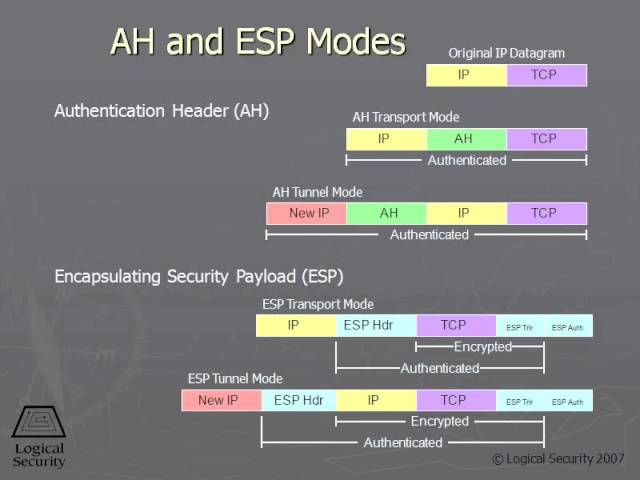
\includegraphics[width=0.86\linewidth]{assets/ipsec_ah_esp_modes.png}

\small\textit{Schéma AH a ESP režimů: AH hlavně autentizuje/integritně chrání, ESP přidává šifrování payloadu; transportní režim chrání původní paket mezi konci, tunelový režim zabalí celý původní IP paket do nového.}
\end{center}

TLS se nachází prakticky mezi transportní a aplikační vrstvou: běží nad TCP a poskytuje bezpečný kanál aplikačním protokolům. Proto vzniká HTTP na HTTPS, FTP na FTPS, případně zabezpečené varianty poštovních protokolů. TLS chrání komunikaci mezi dvěma koncovými body TLS spojení, ověřuje typicky server pomocí certifikátu a po handshake šifruje symetrickým klíčem.

Na aplikační vrstvě existují mechanismy jako PGP nebo S/MIME pro e-mail, aplikační podpisy, tokeny, vlastní autentizační protokoly a aplikační logika. Na linkové vrstvě záleží na technologii: Wi-Fi používá například WPA2/WPA3, podnikové linky mohou mít vlastní linkové zabezpečení, ale není to univerzální ochrana celé internetové cesty.

\itpr{\textbf{Mini box: jak funguje WPA2/WPA3 na Wi-Fi.} WPA chrání bezdrátový úsek mezi klientem a access pointem: nejdřív ověří, že klient zná správné tajemství nebo má správnou identitu, a potom šifruje rámce přenášené vzduchem. U domácího \textbf{WPA2-Personal} mají router i klient stejné heslo/PSK; heslo se neposílá vzduchem, ale použije se při \textbf{4-way handshake}, kde si strany přes nonce odvodí dočasné šifrovací klíče. Data se pak šifrují hlavně pomocí \textbf{AES-CCMP} a kontroluje se integrita, aby útočník nemohl rámce nepozorovaně měnit nebo přehrávat. Slabina WPA2-PSK je, že útočník může zachytit handshake a offline zkoušet hesla ze slovníku. \textbf{WPA3-Personal} nahrazuje PSK handshake metodou \textbf{SAE} (Dragonfly), která je odolnější proti offline hádání hesla a dává každému připojení vlastní klíč s lepší dopřednou bezpečností. Pro firmy je důležitý režim Enterprise, kde se místo sdíleného hesla používá typicky \textbf{802.1X/EAP} a autentizační server.}

VPN znamená virtuální privátní síť. V principu tuneluje provoz přes nedůvěryhodnou síť tak, že mezi klientem a VPN serverem nebo mezi dvěma gatewayemi vznikne chráněný tunel. VPN může chránit důvěrnost a integritu provozu na úseku do VPN brány, umožňuje autentizaci uživatele nebo zařízení a může způsobit, že se klient logicky chová jako součást vzdálené sítě. Neznamená ale automaticky anonymitu ani bezpečnost cílového serveru.

Pokud VPN končí ve firmě, poskytovatel cílové služby stále vidí provoz od VPN brány a aplikace musí být bezpečné samy o sobě.

Firewally filtrují provoz podle pravidel. Paketový filtr pracuje podle IP adres, portů a protokolů na L3/L4. Stateful \textbf{firewall} sleduje stav spojení, takže umí povolit odpovědi k již navázanému spojení. Aplikační firewall nebo NGFW umí kontrolovat obsah aplikačních protokolů, například HTTP, a \textbf{WAF} je specializovaný firewall pro webové aplikace proti útokům jako \textbf{SQL} injection, XSS nebo CSRF.

Proxy funguje jako prostředník: forward \textbf{proxy} řídí odchozí provoz klientů, reverse proxy chrání a zprostředkuje přístup k serverům, často s load balancingem a TLS terminací. \textbf{IDS} útoky detekuje a hlásí, \textbf{IPS} je navíc aktivně blokuje.

Na lokální síti se kromě firewallů uplatňují i ochrany přímo na druhé vrstvě, na switchích. \textbf{DHCP snooping} rozlišuje důvěryhodné a nedůvěryhodné porty a zahazuje DHCP odpovědi z nedůvěryhodných portů, čímž brání podvrženému (rogue) DHCP serveru a omezuje i \textbf{DHCP starvation}, tedy vyčerpání adresního poolu útočníkem. \textbf{Dynamic ARP Inspection} (DAI) kontroluje \textbf{ARP} zprávy proti tabulce z DHCP snoopingu a podvržené zahazuje, čímž brání ARP spoofingu.

Port security omezuje, kolik a jakých \textbf{MAC} adres smí být na portu, a port při porušení zablokuje. Client isolation zabrání tomu, aby spolu klienti na stejné síti, typicky Wi-Fi, navzájem komunikovali. \textbf{VLAN} \textbf{segmentace} odděluje provoz do logických sítí a \textbf{802.1X} vyžaduje autentizaci zařízení nebo uživatele dřív, než se port vůbec zpřístupní.

Dohromady tyto mechanismy řeší útoky, které firewall na hranici sítě nevidí, protože se odehrávají uvnitř jednoho L2 segmentu.

\itbox{\textbf{Vrstvové shrnutí:} Linková vrstva chrání konkrétní linku, IPsec chrání IP komunikaci, TLS chrání kanál pro aplikaci, PGP/S/MIME chrání přímo obsah zprávy. Čím výše zabezpečení leží, tím více rozumí konkrétní aplikaci; čím níže leží, tím transparentnější může být pro aplikace.}

\subsection*{9. Jak bych to celé řekl u státnic}

Síťové aplikace běží na aplikační vrstvě a používají aplikační protokoly, které definují formát, význam a pořadí zpráv. Mezi základní služby patří elektronická pošta, přenos souborů, web a DNS. U pošty se pro odesílání a předávání používá SMTP, zatímco pro vyzvedávání a synchronizaci schránky POP3 nebo IMAP.

U přenosu souborů je klasické FTP nezabezpečené a používá řídicí a datové spojení; FTPS je FTP přes TLS, zatímco SFTP je přenos souborů přes SSH. Web běží nad HTTP, zabezpečená varianta HTTPS používá TLS, které autentizuje server a šifruje komunikaci. DNS je hierarchická distribuovaná služba pro překlad jmen na IP adresy, kde se uplatňuje rekurzivní resolver, root, TLD a autoritativní servery.

Kvalita služby řeší, jaké vlastnosti od přenosu očekáváme: kapacitu, latenci, jitter a ztrátovost. Je důležitá hlavně pro multimédia, VoIP, videokonference a hry, protože ty jsou citlivé na zpoždění a kolísání. Mechanismy QoS zahrnují plánování front, priority, Weighted Fair Queuing, tvarování toků přes Leaky Bucket a Token Bucket a prevenci zahlcení pomocí RED/WRED.

Zabezpečení síťové komunikace řeší důvěrnost, integritu, autentizaci a nepopíratelnost. Symetrická kryptografie je rychlá, ale vyžaduje sdílený klíč; asymetrická kryptografie je pomalejší, ale umožňuje výměnu klíčů a digitální podpisy. V praxi se používá hybridní přístup. Na síťové vrstvě je typický IPsec, mezi transportní a aplikační vrstvou TLS, na aplikační vrstvě například PGP nebo S/MIME.

VPN vytváří chráněný tunel a používá autentizaci a šifrování k ochraně provozu přes nedůvěryhodnou síť.

\subsection*{10. Rychlá kontrola pojmů}

\begin{longtable}{p{0.475\linewidth}p{0.475\linewidth}}
\toprule
\textbf{Oblast} & \textbf{Co říct stručně} \\
\midrule\endhead
SMTP / POP3 / IMAP & SMTP odesílá a předává poštu; POP3 stahuje; IMAP synchronizuje schránku na serveru. \\
\addlinespace
FTP / FTPS / SFTP & FTP je nezabezpečené; FTPS = FTP přes TLS; SFTP = přenos souborů přes SSH; SCP = jednoduché kopírování přes SSH. \\
\addlinespace
DNS & Hierarchie: root, TLD, autoritativní server; rekurzivní resolver dotaz vyřeší a cacheuje. \\
\addlinespace
QoS & Metriky: bandwidth, latence, jitter, ztrátovost; metody: scheduling, token/leaky bucket, RED/WRED. \\
\addlinespace
TLS / IPsec / PGP & TLS chrání kanál aplikace, IPsec IP pakety, PGP/S/MIME obsah e-mailu. \\
\addlinespace
VPN & Tuneluje provoz přes nedůvěryhodnou síť; chrání úsek do VPN brány a autentizuje strany. \\
\addlinespace
\bottomrule
\end{longtable}

\newpage

